\title{504x Project 2: Reinforcement Learning}
\author{Aaron Havens }
\date{\today}
\documentclass[12pt]{article}
\usepackage[margin=1in]{geometry}
\usepackage[tiny,compact]{titlesec}
\usepackage{amssymb} %maths
\usepackage{amsmath} %maths
\usepackage{graphicx}
\usepackage{caption}
\usepackage{subcaption}
\usepackage{verbatim}
\graphicspath{{figs/}}
\begin{document}
\maketitle
\section*{The nature of our learning problem}
In this assignment, we are given three data sets of increasing state and action space. We are not given a transition or reward function, only observations of an agent performing an arbitrary policy (certainly not guaranteed to be optimal). In this way we are strictly learning \textit{Off Policy} meaning that we are learning a policy completely independent of the exploring agent's policy in our data. I do acknowledge that in \textit{small.csv}, since we know the reward states, we may approximate the state transition function with the maximum likelihood of the data, and perform some online methods. However, this method is just as approximate as Q-Learning, which is why I stick to off-line methods in this project.
\section*{Method 1: Q-Learning or Q(0)}
In the \textit{small.csv} data set, all state-action-state triples are sampled at least once. The state-action space is also small (10x10x4). Given this information, achieving convergence with a Q-learning algorithm is extremely straight forward. We start out by constructing a \textit{Q Matrix}, which represents the relative value of taking any action in any state. This implies that our matrix is of dimension 100000x4 and each value is calculated using a temporal difference update (TD) with an eligibility trace of 0. The the policy is extracted by taking the action corresponding the maximum value for a given state.
\begin{align}
Q(s,a) \leftarrow Q(s,a) +\alpha(r_t + \gamma\underset{a}{\text{max}}Q(s_{t+1},a) - Q(s_t,a_t))\\
\pi^*(s) \leftarrow \underset{a}{\text{argmax}} Q(s,a)
\end{align}
where in the max expression, Q is obtained via the Q matrix, $\alpha$ is the learning rate, typically set very low, and $\gamma$ is the discount factor which is given at .95 in this data set. Here is the resulting policy of our grid world.
\section*{Method 2: Stochastic gradient descent with RBF features}
In this case of \textit{medium.csv} and \textit{large.csv} we are dealing with much larger state and action spaces that are not fully sampled. In this case, we must approximate the value of missing state-action-state triples. To do this, I used a stochastic gradient descent(SGD) model paramterized by features. This way we do not have to store a gigantic Q matrix and can estimate the value of any given state-action pair by features. The features were calculated by transforming the states using a non-linear radial basis function (RBF). Basically we perform Q-Learning just as before, but are training our SGD regression model simultaneously. 
\begin{align}
K(x,x^{'}) = \exp(-\frac{||x-x^{'}||}{2\sigma^2})\\
Q(s,a) \leftarrow \text{SGDRegressor}_a(\theta(s))
\end{align}
The results of this method are interesting, although convergence is not achieved given my computation time limitation, it begins to look like something reasonable. The performance is relatively quick and scales well with number of samples. For medium, the run-time is about $10$ minutes per a sweep of the data (100,000 samples) and large takes about $20$ minutes for large (1,000,000 samples).
\section{Resulting figures for Small and Medium}
\begin{figure}[h]
\centering
\begin{subfigure}{.5\textwidth}
  \centering
  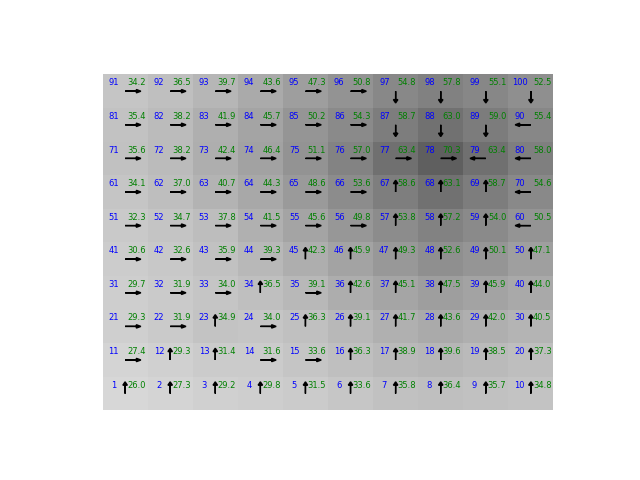
\includegraphics[width=1.2\linewidth]{grid_mdp}
  \caption{Resulting policy visualization of grid-world mdp using Q-learning}
  \label{fig:sub1}
\end{subfigure}%
\begin{subfigure}{.5\textwidth}
  \centering
  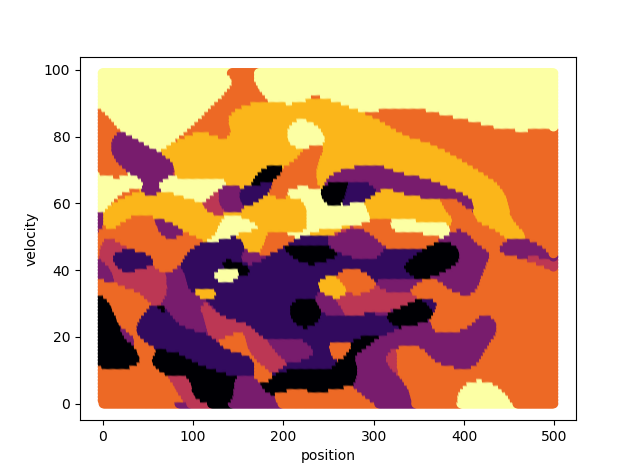
\includegraphics[width=1.2\linewidth]{small}
  \caption{The policy map in position-velocity space where colors represent different actions}
  \label{fig:sub2}
\end{subfigure}
\label{fig:test}
\end{figure}
\appendix
\section{Source Code}
\begin{verbatim}
import matplotlib.pyplot as plt
from math import *
from numpy import genfromtxt
import numpy as np
import matplotlib.patches as patches
import pylab as pylab

#plt.ion()

data_set = 'data/small.csv'
data = genfromtxt(data_set, dtype='int64', delimiter=',',skip_header=True)

def Q_max(Q,s):
	max_r = 0
	for reward in Q[s-1,:]:
		if reward > max_r:
			max_r = reward
	return max_r

def plot_stage(ax,Q):
	grid = np.zeros((10,10))
	index = 0
	reds = plt.get_cmap('Greys')
	max_q = np.max(Q)
	print(max_q)
	min_q = np.min(Q)
	for j in range(10):
		for i in range(10):
			r_m= np.max(Q[index,:])
			ax.add_patch(patches.Rectangle((i-.5, j-.5),1,1,facecolor = reds(r_m/100)))
			grid[i,j] = r_m
			index += 1
	print(grid)
	index = 1
	for j in range(10):
		for i in range(10):
			a = np.argmax(Q[index-1,:])
			ax.text(i+.25, j+.25, "{:.1f}".format(grid[i,j]), ha="center", va="center",size=6,color='g')
			ax.text(i-.25, j+.25, "{:d}".format(index), ha="center", va="center",size=6,color='b')
			if(a == 0):
				ax.arrow(i, j, -.25, 0, head_width=0.1, head_length=0.1, fc='k', ec='k')
			elif(a == 1):
				ax.arrow(i, j, .25, 0, head_width=0.1, head_length=0.1, fc='k', ec='k')
			elif(a == 2):
				ax.arrow(i, j, 0, .25, head_width=0.1, head_length=0.1, fc='k', ec='k')
			elif(a == 3):
				ax.arrow(i, j, 0, -.25, head_width=0.1, head_length=0.1, fc='k', ec='k')
			else:
				ax.arrow(i, j, 0, -.25, head_width=0.1, head_length=0.1, fc='k', ec='k')
				ax.arrow(i, j, 0, .25, head_width=0.1, head_length=0.1, fc='k', ec='k')
				ax.arrow(i, j, .25, 0, head_width=0.1, head_length=0.1, fc='k', ec='k')
				ax.arrow(i, j, -.25, 0, head_width=0.1, head_length=0.1, fc='k', ec='k')
			index += 1
	ax.set_xlim(-1,10)
	ax.set_ylim(-1,10)

def write_policy(q):
	with open('small.policy', 'w') as f:
		for pos in range(100):
			f.write('{}\n'.format(pos,vel,np.argmax(q[i,:])))



gamma = .95
alpha = .01
n_states = 100
n_actions = 4
n_samples = len(data[:,0])
t = 0

s = data[0,0]
Q = np.zeros((n_states,n_actions))
ax = plt.axes()
for k in range(200):
	for i in range(n_samples):
		Q[data[i,0]-1,data[i,1]-1] += alpha*(data[i,2]+gamma*Q_max(Q,data[i,3])-Q[data[i,0]-1,data[i,1]-1])
	print(k)
write_policy(Q)
plot_stage(ax,Q)
plt.axis('off')
plt.show()


import numpy as np
import matplotlib.pyplot as plt
from numpy import genfromtxt
from sklearn.linear_model import SGDRegressor
from sklearn.kernel_approximation import RBFSampler
import sys
import sklearn.pipeline
import sklearn.preprocessing

def decode_state(state):
	vel = state//500
	pos = state%500 - 1
	return [pos, vel]
data_set = 'data/medium.csv'
data = genfromtxt(data_set, dtype='int64', delimiter=',',skip_header=True)
#500*100 possible states, 7 actions for each state.
sample_size = np.size(data[:,0])
episodes = 1
gamma = .5

examples = np.zeros((10000,2))
for i in range(10000):
	examples[i,:] = decode_state(data[i,0])
observation_examples = np.array(examples)
scaler = sklearn.preprocessing.StandardScaler()
scaler.fit(observation_examples)
featurizer = sklearn.pipeline.FeatureUnion([
        ("rbf1", RBFSampler(gamma=5.0, n_components=100)),
        ("rbf2", RBFSampler(gamma=2.0, n_components=100)),
        ("rbf3", RBFSampler(gamma=1.0, n_components=100)),
        ("rbf4", RBFSampler(gamma=0.5, n_components=100))
        ])
featurizer.fit(scaler.transform(observation_examples))
# Used to converte a state to a featurizes represenation.
# We use RBF kernels with different variances to cover different parts of the space
class Estimator():

	def __init__(self,data):

		self.models=[]
		for _ in range(7):
			model = SGDRegressor(learning_rate = "constant")
			model.partial_fit([self.featurize_state(decode_state(data[0,0]))], [0])
			self.models.append(model)
#state = 1 + pos +vel*500
	def featurize_state(self,state):
		scaled = scaler.transform([state])
		featurized = featurizer.transform(scaled)
		return featurized[0]

	def predict(self,s,a=None):
		features = self.featurize_state(s)
		print(np.shape(features))
		if not a:
			return np.array([m.predict([features])[0] for m in self.models])
		else:
			return self.models[a].predict([features])[0]

	def update(self,s,a,y):
		features = self.featurize_state(s)
		self.models[a].partial_fit([features],[y])

def q_learn(data, estimator,episodes,gamma):
	for i in range(episodes):
		for k in range(sample_size):
			state,action,reward,next_state = data[k,:]
			state = decode_state(state)
			next_state = decode_state(next_state)
			q_values_next = estimator.predict(next_state)
			td_step = gamma*np.max(q_values_next)
			td_target = reward + td_step
			estimator.update(state,action-1,td_target)
			print(i)

def write_policy(estimator):
	with open('out_policy_1.txt', 'w') as f:
		for pos in range(500):
			for vel in range(100):
				f.write('{},{},{}\n'.format(pos,vel,np.argmax(estimator.predict([pos,vel]))))


estimator = Estimator(data)
q_learn(data,estimator,10,.99)
write_policy(estimator)

import numpy as np
import matplotlib.pyplot as plt
from numpy import genfromtxt
from sklearn.linear_model import SGDRegressor
from sklearn.kernel_approximation import RBFSampler
import sys
import sklearn.pipeline
import sklearn.preprocessing


data_set = 'data/medium.csv'
data = genfromtxt(data_set, dtype='int64', delimiter=',',skip_header=True)
#500*100 possible states, 7 actions for each state.
sample_size = np.size(data[:,0])
episodes = 1
gamma = .5

examples = np.zeros((10000,1))
for i in range(10000):
	examples[i,0] = data[i,0]
observation_examples = np.array(examples)
scaler = sklearn.preprocessing.StandardScaler()
scaler.fit(observation_examples)
featurizer = sklearn.pipeline.FeatureUnion([
        ("rbf1", RBFSampler(gamma=5.0, n_components=100)),
        ("rbf2", RBFSampler(gamma=2.0, n_components=100)),
        ("rbf3", RBFSampler(gamma=1.0, n_components=100)),
        ("rbf4", RBFSampler(gamma=0.5, n_components=100))
        ])
featurizer.fit(scaler.transform(observation_examples))
# Used to converte a state to a featurizes represenation.
# We use RBF kernels with different variances to cover different parts of the space
class Estimator():

	def __init__(self,data):

		self.models=[]
		for _ in range(8):
			model = SGDRegressor(learning_rate = "constant")
			model.partial_fit([self.featurize_state(data[0,0])], [0])
			self.models.append(model)
#state = 1 + pos +vel*500
	def featurize_state(self,state):
		scaled = scaler.transform([[state]])
		featurized = featurizer.transform(scaled)
		return featurized[0]

	def predict(self,s,a=None):
		features = self.featurize_state(s)
		if not a:
			return np.array([m.predict([features])[0] for m in self.models])
		else:
			return self.models[a].predict([features])[0]

	def update(self,s,a,y):
		features = self.featurize_state(s)
		self.models[a].partial_fit([features],[y])

def q_learn(data, estimator,episodes,gamma):
	for i in range(episodes):
		for k in range(sample_size):
			state,action,reward,next_state = data[k,:]
			q_values_next = estimator.predict(next_state)
			td_step = gamma*np.max(q_values_next)
			td_target = reward + td_step
			estimator.update(state,action-1,td_target)
			print(k)

def write_policy(estimator):
	with open('large.policy', 'w') as f:
		for i in range(1757600):
				f.write('{}\n'.format(np.argmax(estimator.predict(i))))


estimator = Estimator(data)
#print(estimator.featurize_state(decode_state(data[0,0])))
q_learn(data,estimator,1,.99)
write_policy(estimator)
import numpy as np
import matplotlib.pyplot as plt
from numpy import genfromtxt
from sklearn.linear_model import SGDRegressor
from sklearn.kernel_approximation import RBFSampler
import sys
import sklearn.pipeline
import sklearn.preprocessing


data_set = 'data/medium.csv'
data = genfromtxt(data_set, dtype='int64', delimiter=',',skip_header=True)
#500*100 possible states, 7 actions for each state.
sample_size = np.size(data[:,0])
episodes = 1
gamma = .5

examples = np.zeros((10000,1))
for i in range(10000):
	examples[i,0] = data[i,0]
observation_examples = np.array(examples)
scaler = sklearn.preprocessing.StandardScaler()
scaler.fit(observation_examples)
featurizer = sklearn.pipeline.FeatureUnion([
        ("rbf1", RBFSampler(gamma=5.0, n_components=100)),
        ("rbf2", RBFSampler(gamma=2.0, n_components=100)),
        ("rbf3", RBFSampler(gamma=1.0, n_components=100)),
        ("rbf4", RBFSampler(gamma=0.5, n_components=100))
        ])
featurizer.fit(scaler.transform(observation_examples))
# Used to converte a state to a featurizes represenation.
# We use RBF kernels with different variances to cover different parts of the space
class Estimator():

	def __init__(self,data):

		self.models=[]
		for _ in range(8):
			model = SGDRegressor(learning_rate = "constant")
			model.partial_fit([self.featurize_state(data[0,0])], [0])
			self.models.append(model)
#state = 1 + pos +vel*500
	def featurize_state(self,state):
		scaled = scaler.transform([[state]])
		featurized = featurizer.transform(scaled)
		return featurized[0]

	def predict(self,s,a=None):
		features = self.featurize_state(s)
		if not a:
			return np.array([m.predict([features])[0] for m in self.models])
		else:
			return self.models[a].predict([features])[0]

	def update(self,s,a,y):
		features = self.featurize_state(s)
		self.models[a].partial_fit([features],[y])

def q_learn(data, estimator,episodes,gamma):
	for i in range(episodes):
		for k in range(sample_size):
			state,action,reward,next_state = data[k,:]
			q_values_next = estimator.predict(next_state)
			td_step = gamma*np.max(q_values_next)
			td_target = reward + td_step
			estimator.update(state,action-1,td_target)
			print(k)

def write_policy(estimator):
	with open('large.policy', 'w') as f:
		for i in range(1757600):
				f.write('{}\n'.format(np.argmax(estimator.predict(i))))


estimator = Estimator(data)
#print(estimator.featurize_state(decode_state(data[0,0])))
q_learn(data,estimator,1,.99)
write_policy(estimator)
\end{verbatim}
\end{document}